\section{Verfahren zur Ausreißererkennung}
%\subsection{k"=Next"=Neighbors}

\subsection{Isolation Forest}
Das Isolation Forest oder iForest Verfahren zur Ausreißererkennung von Fei Tony Liu et al. \cite{iForest}, erkennt Ausreißer dadurch, dass sie leichter von anderen zu isolieren sind. Isolieren bedeutet hierbei das Abgrenzen eines Punktes von Anderen. Ausreißer sind leichter abzugrenzen, da sie zwei Eigenschaften besitzen:
\begin{enumerate}
    \item "`Ausreißer sind eine Minderheit, die aus wenigen [Datenpunkten] besteht"',
    \item "`Sie besitzen Werte die sich stark von denen, von normalen [Datenpunkten] unterscheiden"',
\end{enumerate}
(vergleiche \cite[Ch. 1]{iForest}, aus dem Englischen übersetzt). \\
iForest isoliert Datenpunkte, indem es sie zufällig partitioniert, so lange bis nur noch ein Datenpunkt in einer Partition liegt. Diese zufällige Partitionierung sorgt dafür, dass Ausreißer mit nur wenigen Partitionen isoliert werden, da es nur wenige Datenpunkte sind, die sich von den anderen stark unterscheiden. Um diese Idee visuell zu verdeutlichen, veranschaulicht die \autoref{fig:partitionierungen} eine Isolierung von einem normalen Datenpunkt $x_i$ und von einem Ausreißer $x_0$. Dabei sind die kleinen Kreise die verschiedenen Datenpunkte und die schwarzen Linien die Grenzen der Partitionen. In \autoref{subfig:partitionierung1} sieht man nun, dass zur Isolierung von $x_i$ viele zufällige Partitionen benötigt werden. In \autoref{subfig:partitionierung2} sieht man wiederum, dass relativ schnell, mit nur zwei zufälligen Partitionen, $x_0$ isoliert werden konnte.
\begin{figure}[bth]
  \subfloat[Isolierung von $x_i$]{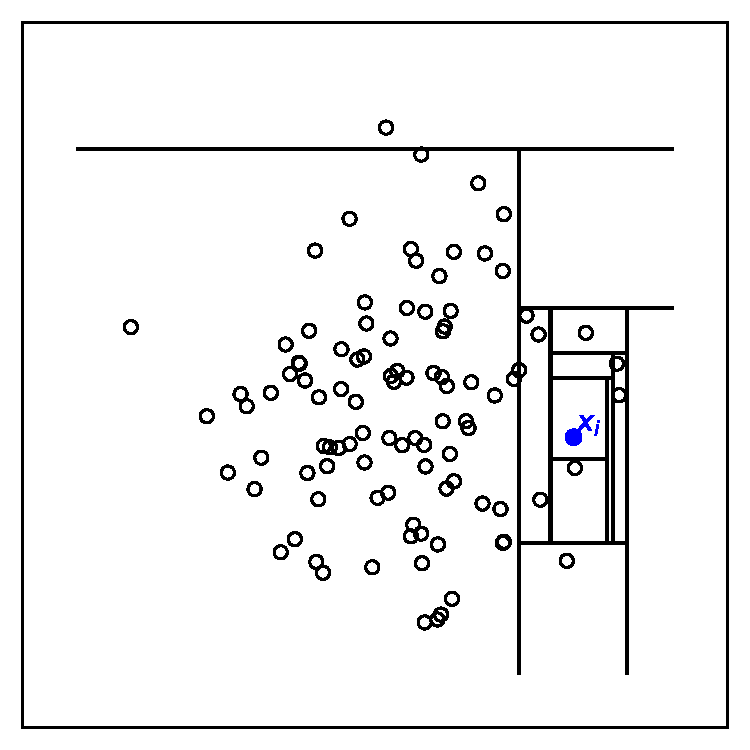
\includegraphics[width=0.49\textwidth]{Graphics/Partitionierung1.pdf}\label{subfig:partitionierung1}}\hfill
  \subfloat[Isolierung von $x_0$]{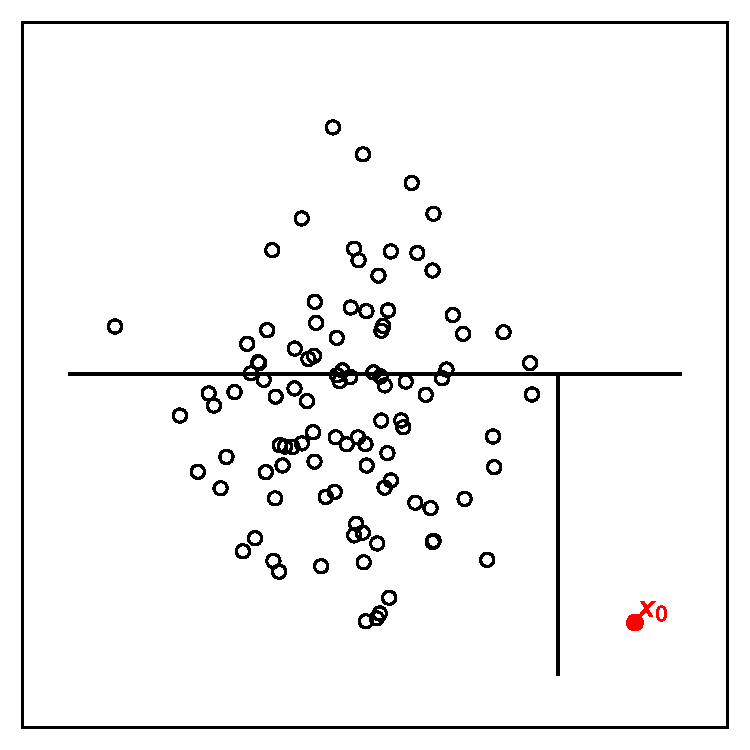
\includegraphics[width=0.49\textwidth]{Graphics/Partitionierung2.pdf}\label{subfig:partitionierung2}}\hfill
  \caption{Zufällige Partitionierung zur Isolierung zweier Punkte, angelehnt an \cite[Fig. 1]{iForest}}
  \label{fig:partitionierungen}
\end{figure}